In order to explain why the proximity of generated samples to the anchor $x$ is relevant to the efficiency during training, 
one can consider a simple example in Euclidean space.
Imagine images as input to a \ac{nn}, which projects them onto $f_{\theta}(x) \in \mathbb{R}^d$, 
where $\theta$ are the parameters of the \ac{nn}.
The effect of the distance between the anchor $x$ and the positive $x^+$ (negative $x^-$) 
sample on the loss is visualized in \autoref{fig:hard_easy_samples_dist_effect_loss}.
Since difficult samples hold more (gradient) information, they have a higher loss value.
Hence, similar negative pairs ($x$, $x^-$) are considered hard \citet{robinson_contrastive_2021}, 
while distant positive pairs ($x$, $x^+$) are considered hard.

% \begin{figure}[h] % h = here, t = top, b = bottom, p = page of floats
%     \centering
%     \includesvg[width=300pt]{images/Hard_easy_samples_dist_effect_loss}
%     \caption{The impact of the distance between a generated sample and its anchor on the loss function.
%     Hard samples convey more (gradient) information than easy samples and thus, have a higher loss value.
%     While distant positive pairs are considered hard, for negative samples, small proximity ones are considered hard.}
%     \label{fig:hard_easy_samples_dist_effect_loss}
% \end{figure}

\begin{figure}[h] % h = here, t = top, b = bottom, p = page of floats
    \centering
    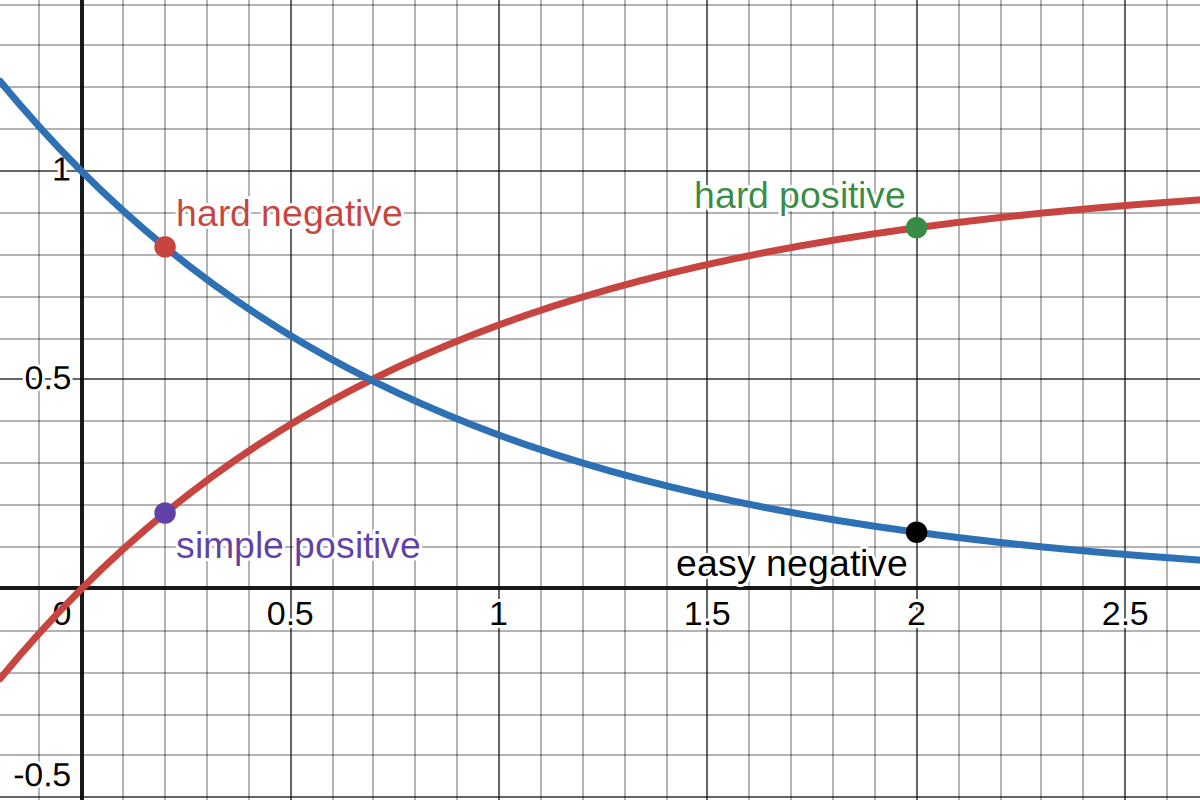
\includegraphics[width=280pt]{images/Hard_easy_samples_dist_effect_loss_desmos.png}
    \caption{The impact of the distance between a generated sample and its anchor on the loss function.
    The red curve represents the loss function for positive samples, 
    whereas the blue curve denotes negative samples.
    Hard samples convey more (gradient) information than easy samples and thus, have a higher loss value.
    While distant positive pairs are considered hard, for negative samples, small proximity ones are considered hard.}
    \label{fig:hard_easy_samples_dist_effect_loss}
\end{figure}